\chapter{Ein Kapitel des Hauptteils}
\section{Verfügbare Daten}
\label{cap:background_sec:setting}
Nun wird die Herkunft der für die nächsten Kapitel elementaren Daten erläutert. Ein Elektrofahrzeug verfügt über folgende Daten, die Ankunftszeit an der Ladestation für den aktuellen Ladezyklus, die Abfahrtszeit, wenn diese erreicht ist endet der aktuelle Ladezyklus. Ebenso gibt jedes Fahrzeug für sich an, ob es gerade verfügbar ist, sprich mit einer Ladestation verbunden ist, welchen Ladezustand der im Fahrzeug verbaute Akku aktuell hat, sowie die aktuell mögliche Ladeleistung. Die Ladegräte wissen jeweils welche Leistung sie gerade an das mit ihnen verbunden Elektrofahrzeug abgeben, sofern den ein Elektrofahrzeug mit ihnen verbunden ist. Einige Daten sind auch aus dem Stromnetz an sich bekannt, so ist die Leistungsabgabe des Transformators ans Stromnetz bekannt, sowie für jeden betrachten Hausanschluss, das dort aktuell vorherrschende Spannungslevel.

\section{VDE 4100 Controller}
\label{cap:background_sec:pureVDE}
Die aktuell im Stromnetz vorliegende Situation, wird durch die Verwendung des Anschlusses ans Stromnetz gemäß der Technischen Anschlussregel Niederspannung(VDE-AR-N 4100) simuliert. Die Anschlussregel gibt vor, wie sich die aktuell anliegende Spannung auf den möglichen Leistungsbezug des Anschlusses auswirkt. \\
\begin{figure}[h!]
	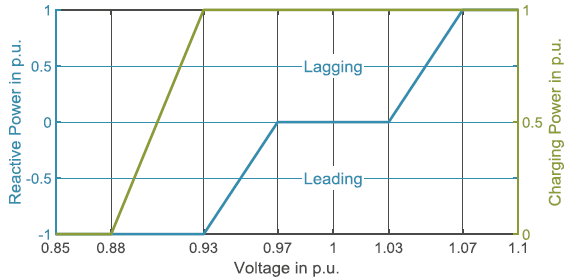
\includegraphics[width=\linewidth]{img/VDEGraph.png}
	\caption{Spannungs zu Leistungsverhältnis nach VDE-AR-N 4100}
	\label{Abb_VDEController}
\end{figure}

\begin{figure}[h!]
	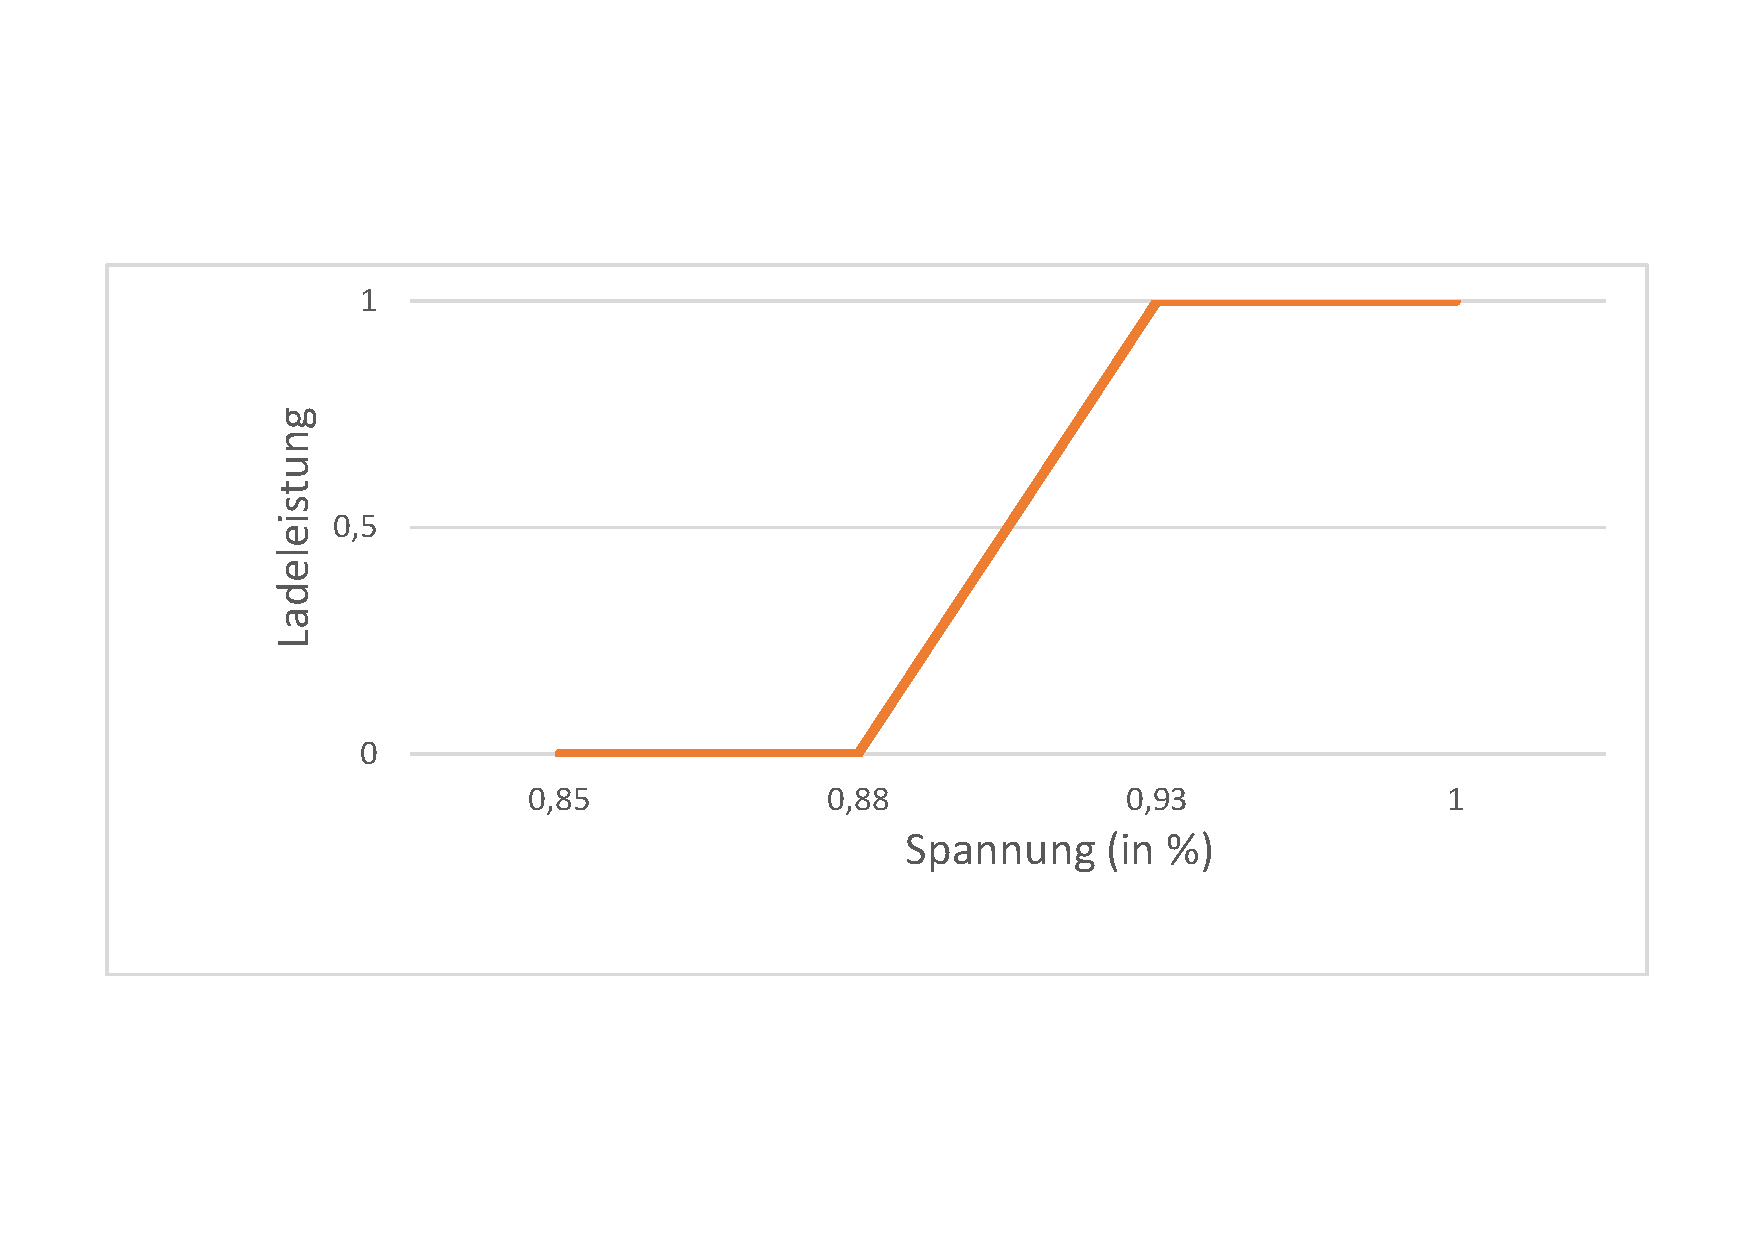
\includegraphics[width=\linewidth]{img/Dia2.pdf}
	\caption{Spannungs zu Leistungsverhältnis nach VDE-AR-N 4100(grün)}
	\label{Abb_VDEController2}
\end{figure}
Per Definition wird von einer Normspannung von 230 Volt ausgegangen. Aus der Abbildung \ref{Abb_VDEController} ist erkennbar, dass wenn weniger als 93\% dieser Normspannung vorliegen, wird die Leistung linear reduziert, wenn der Wert der anliegenden Spannung unter 88\% der Normspannung fällt, wird der Leistungsbezug komplett eingestellt, bis die Spannung wieder auf mindestens 88\% der Normspannung von 230 Volt steigt. Bei einer Spannung zwischen 93\% und 88\% der Normspannung wird der mögliche Leistungsbezug, in diesem Fall die Ladeleistung, linear von voller geforderter Leistung bis zur Abschaltung reduziert.\\
Bis auf die Leistungsreduktion werden von dieser Anschlussregel keine weiteren Maßnahmen getroffen um die Spannung im Netz stabil zu halten. 
Neben der Leistungsreduktion ist es ebenfalls möglich Blindleistung wieder in Stromnetz einzuspeisen um Das Spannungslevel zu erhöhen(Siehe Abbildung \ref{Abb_VDEController}, blaue Kurve), diese Möglichkeit wird aber nicht weiter betrachtet.

\section{Slotted Aloha Ansatz}
\label{cap:background_sec:SA_participants}
Diese Art der Verwendung des Slotted ALOHA Protokolls, definiert eine Kollision, wenn der aktuell vorliegende Spannungswert unter 93\% der Normspannung von 230 Volt fällt. Tritt eine Kollision auf, wird die aktuell anliegende Leistung auf Null reduziert und eine Wartezeit bestimmt, in welcher keine Leistung aus dem Netz bezogen wird. Die Wartezeit wird per Zufall bestimmt, sie wird aus einem Intervall gezogen. Dieses Intervall beginnt  bei Null und wird nach oben von der aktuell Anzahl an Fahrzeugen begrenzt, welche aktuell mit einer beliebigen im Netz installierten Ladestation verbunden sind und Leistung beziehen möchten. Nach dem Ablauf der Wartezeit wird wieder Leistung aus dem Netz bezogen, bis entweder keine Leistung mehr benötigt wird oder wieder eine Kollision auftritt.
Bei dieser Art der Bestimmung der Wartezeit wird weder der aktuelle Ladezustand, noch die verbleibende Zeit des Fahrzeuges am Ladegerät bis zur nächsten Abfahrt berücksichtigt. Lediglich die Zahl der aktuell mit dem Netz verbunden Fahrzeuge, egal ob ladend oder wartend, wird berücksichtigt.

\section{Modifizierter Slotted Aloha Ansatz}
mein Ansatz mit spezieller Wartezeit, Notfallmodus, evtel wieder 4100 und tau filter

